% Options for packages loaded elsewhere
\PassOptionsToPackage{unicode}{hyperref}
\PassOptionsToPackage{hyphens}{url}
%
\documentclass[
]{article}
\usepackage{amsmath,amssymb}
\usepackage{iftex}
\ifPDFTeX
  \usepackage[T1]{fontenc}
  \usepackage[utf8]{inputenc}
  \usepackage{textcomp} % provide euro and other symbols
\else % if luatex or xetex
  \usepackage{unicode-math} % this also loads fontspec
  \defaultfontfeatures{Scale=MatchLowercase}
  \defaultfontfeatures[\rmfamily]{Ligatures=TeX,Scale=1}
\fi
\usepackage{lmodern}
\ifPDFTeX\else
  % xetex/luatex font selection
\fi
% Use upquote if available, for straight quotes in verbatim environments
\IfFileExists{upquote.sty}{\usepackage{upquote}}{}
\IfFileExists{microtype.sty}{% use microtype if available
  \usepackage[]{microtype}
  \UseMicrotypeSet[protrusion]{basicmath} % disable protrusion for tt fonts
}{}
\makeatletter
\@ifundefined{KOMAClassName}{% if non-KOMA class
  \IfFileExists{parskip.sty}{%
    \usepackage{parskip}
  }{% else
    \setlength{\parindent}{0pt}
    \setlength{\parskip}{6pt plus 2pt minus 1pt}}
}{% if KOMA class
  \KOMAoptions{parskip=half}}
\makeatother
\usepackage{xcolor}
\usepackage[margin=1in]{geometry}
\usepackage{graphicx}
\makeatletter
\def\maxwidth{\ifdim\Gin@nat@width>\linewidth\linewidth\else\Gin@nat@width\fi}
\def\maxheight{\ifdim\Gin@nat@height>\textheight\textheight\else\Gin@nat@height\fi}
\makeatother
% Scale images if necessary, so that they will not overflow the page
% margins by default, and it is still possible to overwrite the defaults
% using explicit options in \includegraphics[width, height, ...]{}
\setkeys{Gin}{width=\maxwidth,height=\maxheight,keepaspectratio}
% Set default figure placement to htbp
\makeatletter
\def\fps@figure{htbp}
\makeatother
\setlength{\emergencystretch}{3em} % prevent overfull lines
\providecommand{\tightlist}{%
  \setlength{\itemsep}{0pt}\setlength{\parskip}{0pt}}
\setcounter{secnumdepth}{-\maxdimen} % remove section numbering
\usepackage{booktabs}
%\usepackage[utf8]{inputenc}
%\usepackage{mathptmx}
%\usepackage{newtxtext,newtxmath}
\usepackage{xunicode} % Unicode support for LaTeX character names (accents, European chars, etc)
\usepackage{xltxtra} % Extra customizations for XeLaTeX
%\setmainfont{Crimson Pro} % set the main body font (\textrm)
%\setsansfont{Source Sans Pro}
%\setmonofont{Ubuntu Mono}

\addtolength{\topmargin}{-1cm}
\addtolength{\textheight}{3cm}
\addtolength{\oddsidemargin}{-1cm}
\addtolength{\textwidth}{2cm}


\DeclareMathOperator*{\argmin}{argmin}
\DeclareMathOperator*{\logit}{logit}
\DeclareMathOperator*{\expit}{expit}
\newcommand{\var}{\mathrm{Var}}
\newcommand{\bfa}[2]{{\rm\bf #1}[#2]}
\newcommand{\rma}[2]{{\rm    #1}[#2]}
\newcommand{\estm}{\widehat}

% <!--- For HTML Only --- Equivalent code for .pdf must be included in preamble.tex -->
% `r if (!knitr:::is_latex_output()) '
% $\\DeclareMathOperator*{\\argmin}{argmin}$
% $\\DeclareMathOperator*{\\logit}{logit}$
% $\\DeclareMathOperator*{\\expit}{expit}$
% $\\newcommand{\\var}{\\mathrm{Var}}$
% $\\newcommand{\\bfa}[2]{{\\rm\\bf #1}[#2]}$
% $\\newcommand{\\rma}[2]{{\\rm     #1}[#2]}$
% $\\newcommand{\\estm}{\\widehat}$'`
\usepackage{booktabs}
\usepackage{longtable}
\usepackage{array}
\usepackage{multirow}
\usepackage{wrapfig}
\usepackage{float}
\usepackage{colortbl}
\usepackage{pdflscape}
\usepackage{tabu}
\usepackage{threeparttable}
\usepackage{threeparttablex}
\usepackage[normalem]{ulem}
\usepackage{makecell}
\usepackage{xcolor}
\ifLuaTeX
  \usepackage{selnolig}  % disable illegal ligatures
\fi
\IfFileExists{bookmark.sty}{\usepackage{bookmark}}{\usepackage{hyperref}}
\IfFileExists{xurl.sty}{\usepackage{xurl}}{} % add URL line breaks if available
\urlstyle{same}
\hypersetup{
  pdftitle={HAB model},
  hidelinks,
  pdfcreator={LaTeX via pandoc}}

\title{HAB model}
\author{}
\date{\vspace{-2.5em}2024-04-02}

\begin{document}
\maketitle

\hypertarget{model}{%
\subsection{Model}\label{model}}

\begin{itemize}
\item
  \(n\) polygons \(i=1,\ldots,n\)
\item
  \(t\) time in weeks: Week 0 is the week of 1 January 2018
\item
  \(q_t\) is the seasonal indicator: 1 if the week is in the months of
  December-July, 0 otherwise
\item
  \(V_i\) volume to a depth of 15m
\item
  \(P_{ijt}\) = proportion of mass in polygon \(j\) moving to polygon
  \(i\) in week \(t\).

  Mass conservation implies \[ 
    \sum_{i=1}^n P_{ijt}\leq 1 \qquad\text{for all $j,t$}
  \] where the sum is less than 1 when mass is lost at the edges of the
  set of polygons.
\item
  \(R_{it} \equiv P_{iit}\) = proportion of mass remaining resident in
  week \(t\)
\item
  \({\bf x}_{it}\) covariates in polygon \(i\) at time \(t\)
  (temperature, salinity, etc.)
\item
  At time step \(t\) the epoch indicator \(E_t|E_{t-1}\) is drawn
  \begin{eqnarray*}
     E_0           &\sim& \text{Bernoulli}(\mbox{$\frac12$})\\
     E_t|E_{t-1}=0 &\sim& \text{Bernoulli}(\tau_0 q_t)\qquad\text{for $t>0$}\\
     E_t|E_{t-1}=1 &\sim& \text{Bernoulli}(\tau_1 q_t)
  \end{eqnarray*} where \(\tau_0\) is the probability of initiation of
  an epoch favourable to algal blooms (\(\tau_0\) is low), and
  \(\tau_1\) is the probability of the persistence of that epoch.
\item
  \(\pi_{it}\) bloom initiation probability in polygon \(i\) at time
  \(t\) \[
     \logit(\pi_i) = a_0 + b_0 \logit(R_{it})
  \]
\item
  At time step \(t\) in each polygon \(i\) the innovation indicator is
  drawn \[
     I_{it} \sim \text{Bernoulli}(\pi_{it}E_t)
  \] An innovation in biomass only occurs in a polygon if \(t\) is in a
  favourable epoch (\(E_t\neq 0\)).
\item
  New biomass innovation in polygon \(i\) at time \(t\)
  \begin{eqnarray*}
     A_{it} | I_{it}=0 &\sim& \delta_0\\
     A_{it} | I_{it}=1 &\sim& \Gamma(a,b)
  \end{eqnarray*}
\item
  Time evolution of algal mass \(M_{it}\) \[
     M_{it} = A_{it} + e^{\alpha_{E_t} + {\bf x}_{it}^T{\beta}_2 + \lambda_2 \logit R_{it}}
                       \sum_{j=1}^n P_{ijt} 
                                    e^{{\bf x}_{jt}^T{\beta}_1 + \lambda_1 \logit R_{jt}}
                                    X_{j,t-1}
  \] We may not need both of \(({\beta}_1,\lambda_1)\) (growth before
  transport) and \(({\beta}_2,\lambda_2)\) (growth after transport).
\item
  Observation of algal density \(Y_{it}\) \begin{eqnarray*}
    Y_{it} | M_{it} = 0 &\sim& \delta_0\\
    \log Y_{it} | M_{it}>0, \sigma_\varepsilon^2 &\sim& \text{Normal}(\log M_{it}, \sigma_\varepsilon^2)
  \end{eqnarray*}
\end{itemize}

\begin{verbatim}
## Warning: attribute variables are assumed to be spatially constant throughout
## all geometries
\end{verbatim}

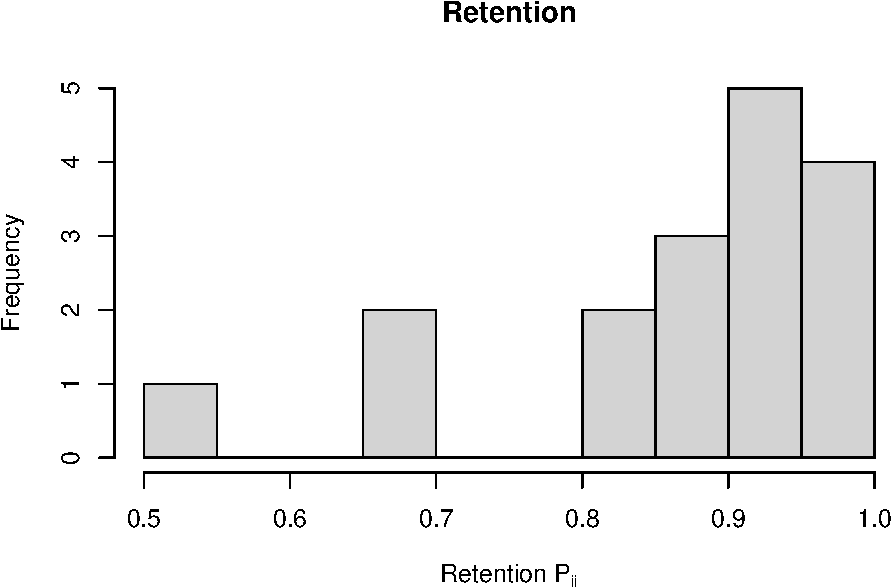
\includegraphics{habmodel_files/figure-latex/unnamed-chunk-2-1.pdf}

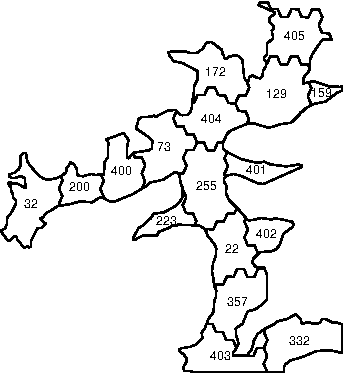
\includegraphics{habmodel_files/figure-latex/unnamed-chunk-3-1.pdf}
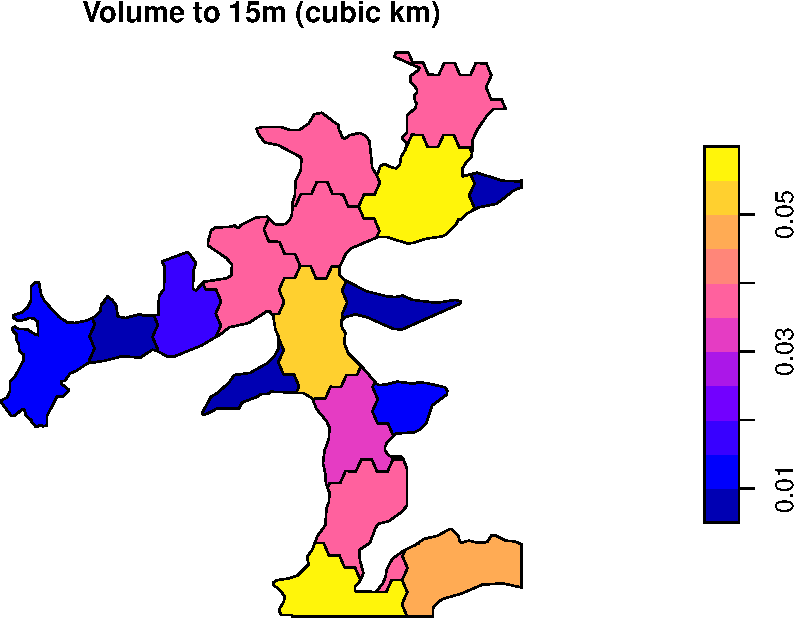
\includegraphics{habmodel_files/figure-latex/unnamed-chunk-3-2.pdf}
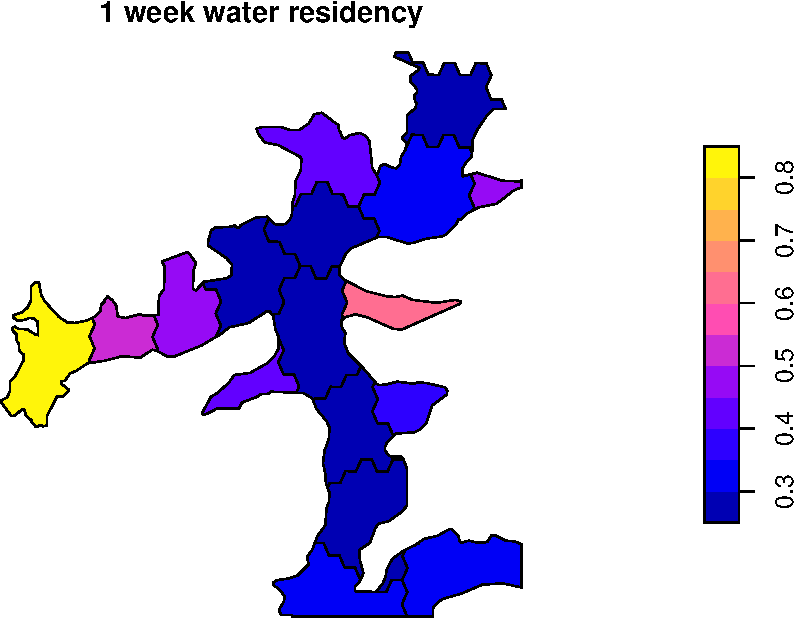
\includegraphics{habmodel_files/figure-latex/unnamed-chunk-3-3.pdf}

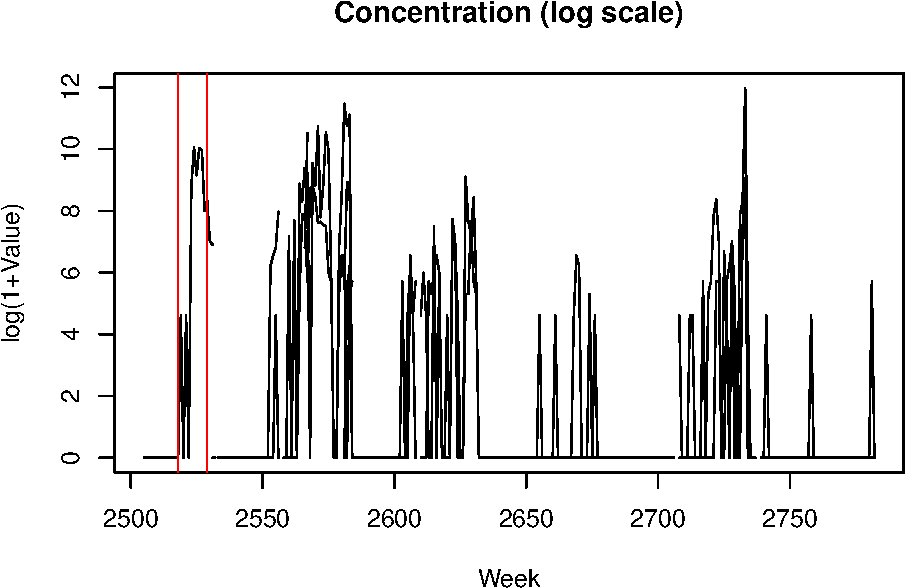
\includegraphics{habmodel_files/figure-latex/unnamed-chunk-5-1.pdf}
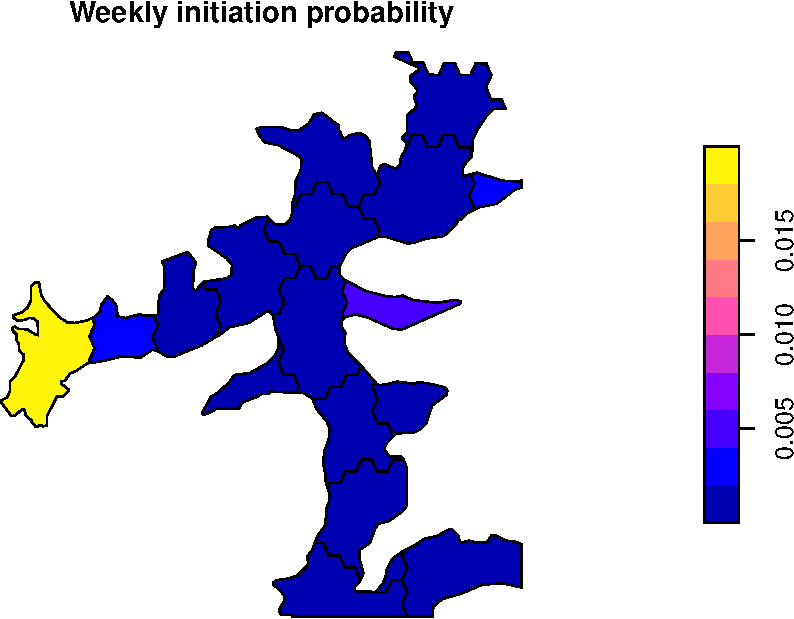
\includegraphics{habmodel_files/figure-latex/unnamed-chunk-5-2.pdf}

\begin{verbatim}
##  [1] 0 2 0 0 1 0 0 1 1 0 0 0 2 0 0 1 0
\end{verbatim}

\begin{verbatim}
## Warning: st_centroid assumes attributes are constant over geometries
\end{verbatim}

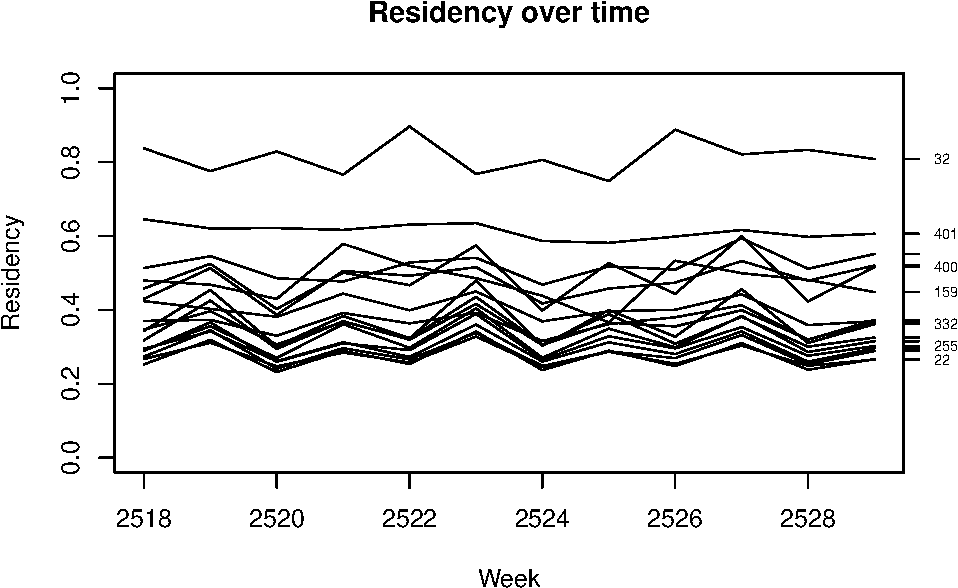
\includegraphics{habmodel_files/figure-latex/unnamed-chunk-6-1.pdf}

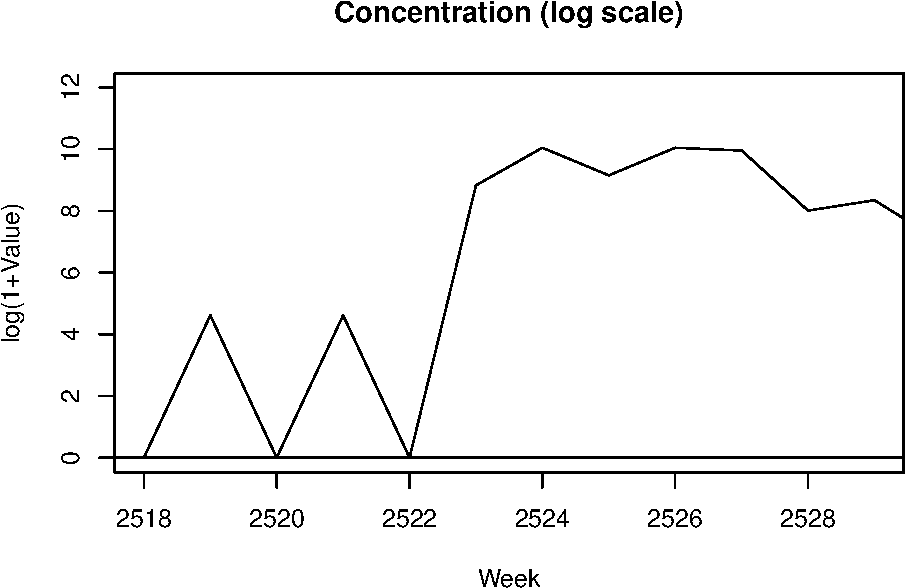
\includegraphics{habmodel_files/figure-latex/unnamed-chunk-7-1.pdf}

\end{document}
